\begin{frame}{Activité: le plus court chemin}
  
  \begin{block}{Matériel nécessaire}
    \begin{itemize}
    \item Une planche avec des trous au hasard,
    \item autant de longs clous que de trous,
    \item une ficelle suffisamment longue et \alert{qui ne soit pas élastique},
    \item un marqueur.
    \end{itemize}
  \end{block}

  \begin{block}{Règles du jeu}
    \begin{itemize}
    \item \structure{Situation initiale :} les clous sont mis dans les trous, leurs têtes dépassent de la planche, et un bout de la ficelle est attachée à un clou.
    \item \structure{Comment jouer :} faire passer la ficelle \alert{une fois et une seule} par \alert{tous les clous} de la planche, puis revenir au point de départ.
    \item  \structure{Objectif :} obtenir le chemin le plus court possible. À chaque fois qu'un record est battu, on fait une marque sur la ficelle pour le mémoriser.
    \end{itemize}
  \end{block}

  \begin{center}
    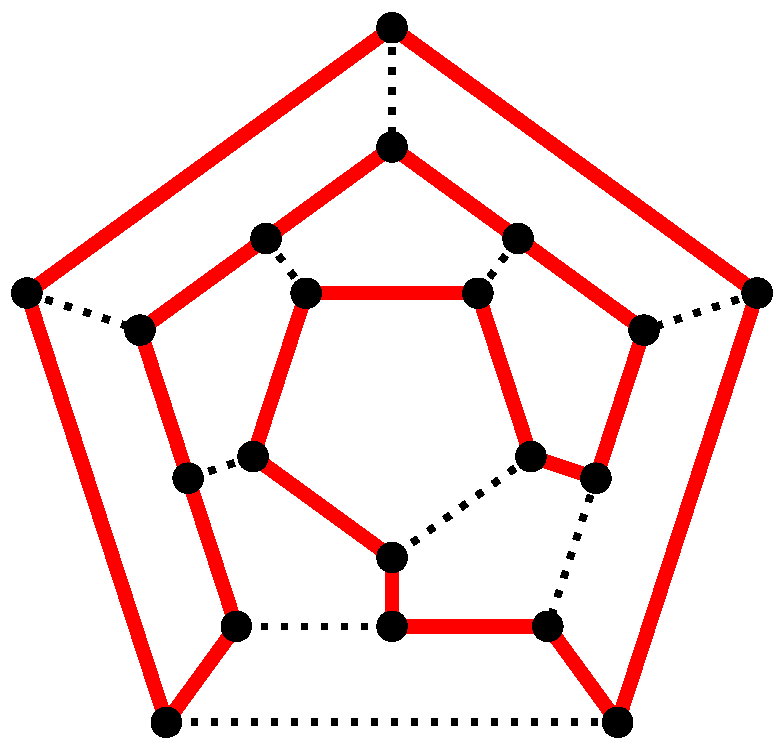
\includegraphics[width=0.3\linewidth]{img/Hamiltonian_path.pdf}
  \end{center}

  \begin{block}{Objectif de l'activité}
    \begin{itemize}
    \item On peut construire un très grand nombre de chemins différents (pour $10$ clous, $10! = 10 \cdot 9 \cdot 8 \cdot \ldots \cdot 2 = 3628800$), et il est très difficile de trouver le meilleur chemin à coup sûr.
    \item A la place, on va chercher des méthodes (algorithmes) pour construire des chemins courts, et comparer leurs résultats.
    \end{itemize}
  \end{block}

\end{frame}

\begin{frame}{Ce qu'il faut retenir du plus court chemin}
  %\centerline{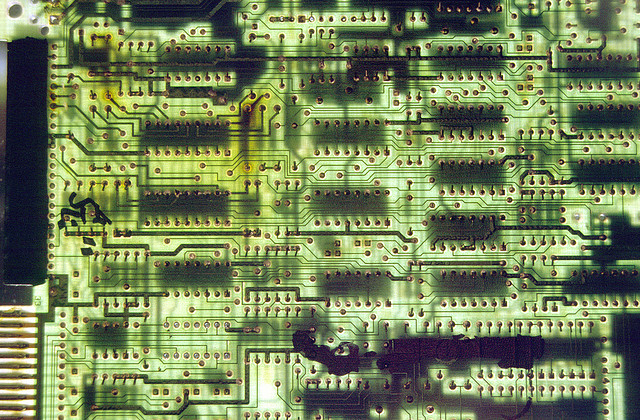
\includegraphics[width=.7\linewidth]{img/electric_city.jpg}\label{img:electric:city}}
  
  \begin{itemize}
    \item Certains problèmes (dont le problème du plus court chemin) sont trop compliqués pour trouver la \alert{solution optimale} en un temps \alert{raisonnable}. Dans de telles situations, on préfère souvent trouver une solution approchée très rapidement, plutôt que de chercher très longtemps la solution optimale. Les méthodes utilisée pour trouver rapidement des solutions approchées sont des \alert{heuristique}.
    \item Le problème du chemin le plus court parait bête mais il fait très difficile, et a de très nombreuses applications dans la vie de tous les jours (comment minimiser la tournée du facteur, la longueur des pistes d'un circuit imprimé, les déplacements d'un bras robotique ...).
  \end{itemize}

  \begin{block}{Trouver la solution optimale}
    
    \begin{itemize}
      \item Dans le cas du chemin le plus court, l'approche naïve consiste à calculer la longueur de tous les chemins et comparer les résultats pour trouver le plus court. La complexité d'une telle approche s'écrit $O(n!)$. Il existe cependant des algorithmes plus efficaces - par exemple, l'algorithme de Held-Karp a une complexité de $O(n^{2}2^n)$. Voici une petite comparaison de l'augmentation de la quantité de calculs nécessaires à mesure que $n$ augmente :

      \bigskip

      \begin{center}
        \begin{tabular}{|l|cccc|}
          \hline
          nombre de sommets       & 5   & 10      & 15            & 20 \\
          \hline
          méthode naïve $O(n!)$   & 120 & 3628800 & 1307674368000 & 2432902008176640000 \\
          Held-Karp $O(n^{2}2^n)$ & 800 & 102400  & 7372800       & 419430400 \\
          \hline
        \end{tabular} 
      \end{center}

      \bigskip

      \item Ce tableau nous montre qu'avec la méthode naïve, en testant un milliard de chemins par seconde, il faudrait plus de \textbf{77 ans} pour trouver le chemin le plus court entre 20 sommets ! En comparaison, l'algorithme Held-Karp met moins d'\textbf{une demi seconde} pour trouver le même résultat !
% les chercheurs classent les problèmes en fonction de la difficulté à trouver des algorithmes efficaces 
    \end{itemize}
  \end{block}

  \begin{center}
    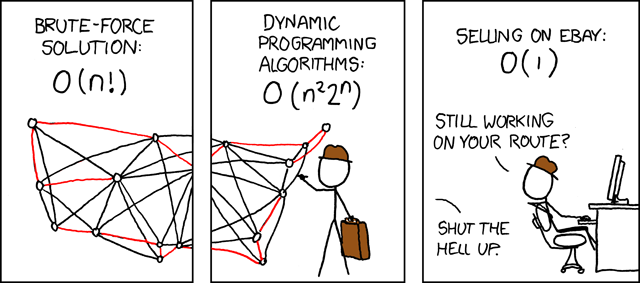
\includegraphics[width=0.8\linewidth]{img/tsp_xkcd.png}
  \end{center}

\end{frame}

\begin{frame}{Ce qu'il faut retenir du plus court chemin}

  \begin{block}{Trouver une solution approchée}


  \end{block}

\end{frame}

    %\item algos NP, NP-difficiles, NP-complets
    %\item C'est un problème qui parait bête mais qui est complexe et qui a de nombreuses applications dans la vie réelle
    %\item Exemple d'application amusante de notion de NP-complétude:  \url{http://arxiv.org/abs/1203.1895}
